\section{PS4a: CircularBuffer}\label{sec:ps4a}
\graphicspath{{ps4a}}
\subsection{Discussion:}\label{sec:ps4a:disc}
 The ps4a assignment creates a circular buffer which will be used for the follow up assignment ps4b. In this assignment, we create basically a circular queue, where the head and tail will be connected and follows the same mechanism as queue i.e, FIFO (First In First Out) Mechanism. 
 \begin{figure}[h]
    \centering
    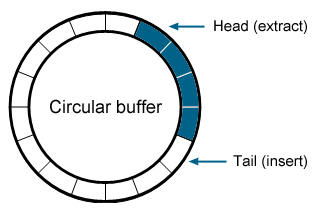
\includegraphics[width=1\textwidth]{ps4a/cb.jpg}
    \caption{Circular Buffer}
    \label{fig:cb}
\end{figure}
\subsection{Key algorithms, Data structures and OO Designs used in this Assignment:}
 I make use of Vectors in standard manner rather than the functions as I found it amusing and easy to understand theoratically, Where I used basic rules such as initial head, tail.
 I used the default format of the pdf to create the template version and also added few functions such as print etc.
 I used exceptions to inform the provided arised exceptions.

\subsection{What I accomplished :}

I have created a CircularBuffer using the vector. It works properly and gives the output too in the main function. I have used the templates so therefore there is no need for .cpp file. 

\subsection{What I already knew :}

I knew how to implement template. I was aware of the CircularBuffer concept as I did a Circular buffer program without using templates in my Data Structure Class.

\subsection{What I learned :}

I learnt how to implement vector and the template in an efficient way.

\subsection{Challenges :}

To implement template throughout the code as well as implementing in the test file was quite a challenge for me.

\subsection{Codebase}\label{sec:ps4a:code}

\textbf{\colorbox{pink}{Makefile:}} \newline \textbf{This Makefile has linting included.}

\lstinputlisting[language=Make]{ps4a/Makefile}

\textbf{\colorbox{pink}{CircularBuffer.h:}} \newline \textbf{This file is the important file as it contains all the methods for the CircularBuffer to run. It does not have a cpp file as I have utilized the template.}
\lstinputlisting{ps4a/CircularBuffer.h}

\textbf{\colorbox{pink}{main.cpp:}} \newline \textbf{This file is just for the output of the sample input and methods of the CircularBuffer}
\lstinputlisting{ps4a/main.cpp}

\newpage
\textbf{\colorbox{pink}{test.cpp: }} \newline \textbf{The test file tests for the Exceptions as well as all the functions of the CircularBuffer as you can see in the output section.}
\lstinputlisting{ps4a/test.cpp}

\subsection{Output :}
\begin{figure}[h]
   \centering
    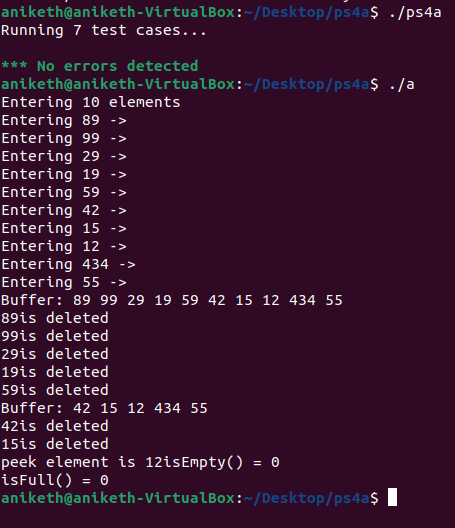
\includegraphics[width=1\textwidth]{ps4a/ps4a.png}
    \caption{PS4a Output in Terminal}
    \label{fig:ps4a}
\end{figure}


\newpage
